\documentclass[a4paper,12pt]{article}
\usepackage[utf8]{inputenc}
\usepackage{graphicx}
\usepackage{tikz}
\usetikzlibrary{shapes.geometric, arrows, positioning}

% Estilos para o fluxograma
\tikzstyle{startstop} = [rectangle, rounded corners, minimum width=3cm, minimum height=1cm, text centered, draw=black, fill=red!30]
\tikzstyle{process} = [rectangle, minimum width=3cm, minimum height=1cm, text centered, draw=black, fill=orange!30]
\tikzstyle{decision} = [diamond, minimum width=3cm, minimum height=1cm, text centered, draw=black, fill=green!30]
\tikzstyle{io} = [trapezium, trapezium left angle=70, trapezium right angle=110, minimum width=3cm, minimum height=1cm, text centered, draw=black, fill=blue!30]
\tikzstyle{textblock} = [rectangle, minimum width=3cm, minimum height=1cm, text centered, draw=black, fill=blue!10]
\tikzstyle{arrow} = [thick,->,>=stealth]

\title{Fluxograma: Madagascar}
\author{
    Diego Nascimento dos Santos \\
    Autor 2
}
\date{18 de outubro de 2024}

\begin{document}

\maketitle

\begin{abstract}
Programa: Jogo da sobrevivência

O programa Madagascar traz um jogo cheio de emoção para o usuário. Neste artigo iremos
apresentar o fluxograma do jogo.

Após essa modelagem de fluxograma será implementado o jogo em linguagem C.

Local: Escola Politécnica de Pernambuco - UPE/POLI \\
Órgão financiador: N/A \\
Caracterização: Modelagem, projeto e implementação em linguagem C
\end{abstract}

\section{Introdução}

O programa será modelado em fluxograma em uma primeira fase, em seguida
sua lógica será desenvolvida em formato de algoritmo, para então
na terceira fase ser implementado em Linguagem de Programação C.

\section{Fluxograma}

\begin{center}
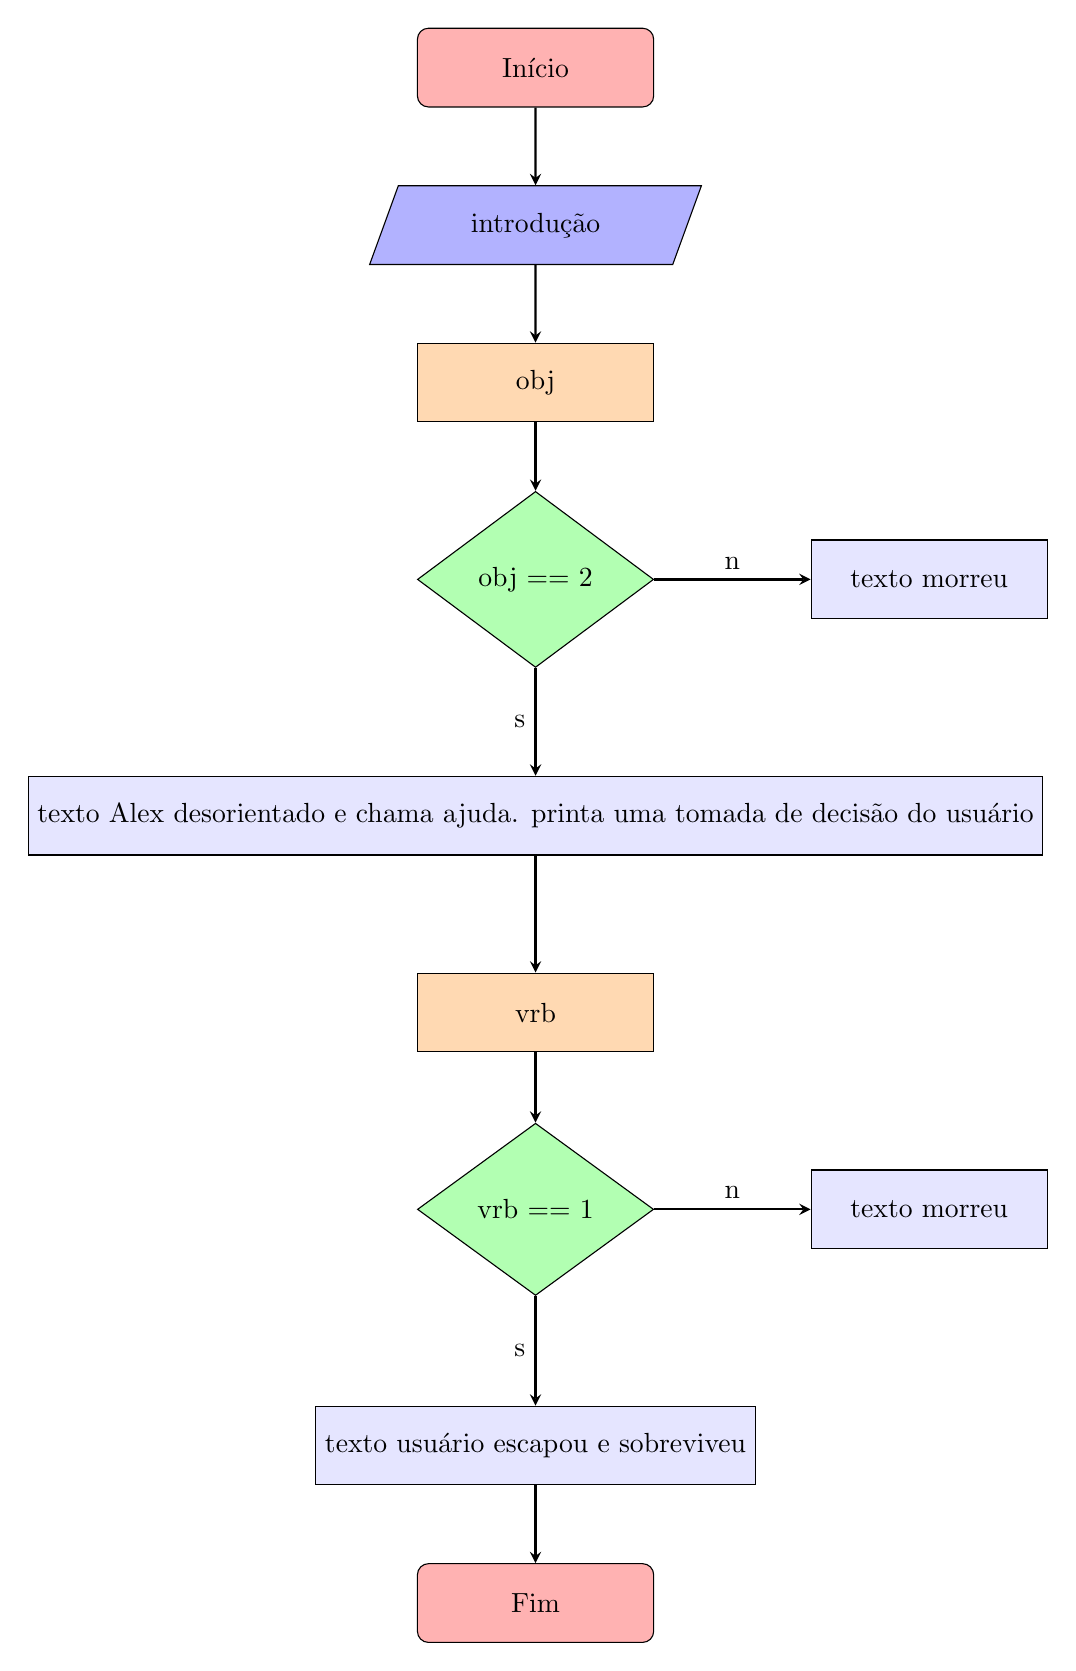
\begin{tikzpicture}[node distance=2cm]

    % Nós
    \node (start) [startstop] {Início};
    \node (intro) [io, below of=start] {introdução};
    \node (obj) [process, below of=intro] {obj};
    \node (dec1) [decision, below of=obj, yshift=-0.5cm] {obj == 2};
    \node (text1) [textblock, right of=dec1, xshift=3cm] {texto morreu};
    \node (alex) [textblock, below of=dec1, yshift=-1cm] {texto Alex desorientado e chama ajuda. printa uma tomada de decisão do usuário};
    \node (vrb) [process, below of=alex, yshift=-0.5cm] {vrb};
    \node (dec2) [decision, below of=vrb, yshift=-0.5cm] {vrb == 1};
    \node (text2) [textblock, right of=dec2, xshift=3cm] {texto morreu};
    \node (escape) [textblock, below of=dec2, yshift=-1cm] {texto usuário escapou e sobreviveu};
    \node (end) [startstop, below of=escape] {Fim};

    % Setas
    \draw [arrow] (start) -- (intro);
    \draw [arrow] (intro) -- (obj);
    \draw [arrow] (obj) -- (dec1);
    \draw [arrow] (dec1) -- node[anchor=south] {n} (text1);
    \draw [arrow] (dec1) -- node[anchor=east] {s} (alex);
    \draw [arrow] (alex) -- (vrb);
    \draw [arrow] (vrb) -- (dec2);
    \draw [arrow] (dec2) -- node[anchor=south] {n} (text2);
    \draw [arrow] (dec2) -- node[anchor=east] {s} (escape);
    \draw [arrow] (escape) -- (end);

\end{tikzpicture}
\end{center}

\section{Detalhamento dos Autores}

\subsection{Discentes}

\begin{itemize}
    \item Nome completo: Diego Nascimento dos Santos
    \item Email: \texttt{dns@upe.br}
    \item Endereço: R. 14, nº 16; Alameda-Paulista - Paulista-PE
    \item Matrícula: CA0211-1
    \item CPF: 113.367.974-95
    \item RG: 10.128-200
    \item Telefone: (81) 9 8692-4449
    \item Currículo Lattes:
\end{itemize}

\begin{itemize}
    \item Nome completo:
    \item Email: \texttt{}
    \item Endereço:
    \item Matrícula:
    \item CPF:
    \item RG:
    \item Telefone:
    \item Currículo Lattes:
\end{itemize}

\subsection{Docentes}

\begin{itemize}
    \item Nome completo: Ruben Carlo Benante
    \item Email: \texttt{rcb@upe.br}
    \item Matrícula: 11238-0
    \item Currículo Lattes: \url{http://lattes.cnpq.br/3366717378277623}
\end{itemize}

\end{document}
